\documentclass[12pt]{article}

% --- PAQUETES NUEVOS PARA EL ALGORITMO ---
\usepackage{algorithm}
\usepackage{algorithmic}
% Para que el título del algoritmo aparezca en español ("Algoritmo" en lugar de "Algorithm")
\floatname{algorithm}{Algoritmo}

\input{../../_assets/preambulo.tex}
% Define a custom command for email addresses
\newcommand{\email}[1]{\href{mailto:#1}{{{\color{blue}#1}}}}
\newcommand{\CD}{CD(G, K) }
\newcommand{\CV}{CV(G, J) }
\newcommand{\ALG}{ALG(G, J) }

% Para poder incluir árboles
\usepackage{forest}
\usepackage{booktabs}


\fancyhead[L]{\helv \nouppercase{\leftmark}}
% \fancyhead[R]{\helv \nouppercase{\rightmark}}

\title{\textbf{Modelos Avanzados\\de Computación}}

\date{}  % Fecha actual

\begin{document}

    % Crear la portada
    \maketitle

    % Subtítulo (puede usarse \Large para hacer el texto más grande)
    \begin{center}
        \LARGE Trabajo de NP-completitud\\Problema del Conjunto Dominante
    \end{center}

    \vspace{1cm}

    \begin{center}
        \large Curso 2025-2026
    \end{center}
    
    \vspace{7cm}

    % Autores
    \begin{center}
        \textbf{José Juan Urrutia Milán} \\ 
        \vspace{1em}  % Espacio entre autores
        Grupo A1
    \end{center}

    \newpage

    \section{Descripción del Problema}
    \noindent
    Describimos a continuación el problema del Conjunto Dominante (CD):
    \begin{itemize}
        \item \textbf{Entrada:} Un grafo $G = (V,E)$ y $K\in \mathbb{N}$ con $K\leq |V|$.
        \item \textbf{Decisión:} Determinar si existe $V'\subseteq V$ con $|V'|\leq K$ y tal que:
            \begin{equation*}
                \forall v\in V\setminus V' ~~\exists u\in V' ~~\text{de forma que}~~ (v,u)\in E \lor (u,v)\in E
            \end{equation*}
    \end{itemize}
    Así, notaremos por \CD a una instancia del problema.

    \section{Demostración de NP-completitud}
    \subsection{Parte 1}
    \noindent
    En primer lugar hemos de probar que CD es un problema de NP. Para ello, el siguiente Algoritmo~\label{alg} puede implementarse en una Máquina de Turing no Determinista.\\

    \noindent
    Este algoritmo primero construye de forma no determinista y en tiempo $O(|V|)$ el conjunto $V'$ y luego comprueba que tenga un tamaño menor o igual que $K$. Posteriormente comprueba en tiempo $O(|V|\cdot K\cdot |E|)$ que $V'$ sea un conjunto dominante, para cada vértice $v\in V$:
    \begin{itemize}
        \item bien $v\in V'$, en cuyo caso al recorrer los vértices $u\in V'$ encontraremos $u = v$, de donde \texttt{encontrado} = \textbf{true} y no necesitamos verificar nada más para este vértice $v$.
        \item bien $v\in V\setminus V'$, en cuyo caso al recorrer $u\in V'$ siempre mantendremos $\texttt{encontrado}$ = \textbf{false}. Al recorrer $e\in E$ hay dos posibilidades:
            \begin{itemize}
                \item bien algún $e = (u,v)$ ó $e = (v,u)$, en cuyo caso se pondrá en algún momento \texttt{conectado} = \textbf{true}.
                \item bien se mantendrá \texttt{conectado} = \textbf{false}, pues no encontraremos una arista de dicha forma, de donde el algoritmo terminará y dirá NO.
            \end{itemize}
    \end{itemize}
    Así, hemos visto que el algoritmo es \underline{correcto}. Además, sea $n$ la longitud total de la entrada al algoritmo, CD exige que $K\leq |V|$ y tendremos que $|V|, |E| \leq n$, de donde el algoritmo tiene orden temporal $O(n^3)$, por lo que el problema es NP.
    \begin{algorithm}
        \caption{}\label{alg}
        \begin{algorithmic}
            \STATE \textbf{Entrada:} La codificación de un grafo $G=(V,E)$ y un número $K\leq |V|$ en binario.\\

            \noindent
            \STATE $V' = \{\}$
        \STATE \textbf{Para cada} vértice $v\in V$ \textbf{hacer}
            \STATE \quad Elegir de forma no determinista si incluir $v$ en $V'$.
            \STATE \textbf{Fin Para}
            \STATE \textbf{Si} tamaño($V'$) $> K$ \textbf{entonces }Terminar algoritmo y decir ``NO''.\\

            \noindent
            \STATE \textbf{Para cada} vértice $v\in V$ \textbf{hacer}
            \STATE \quad \texttt{encontrado} = \textbf{false}
            \STATE \quad \texttt{conectado} = \textbf{false}\\

            \noindent
            \STATE \quad \textbf{Para cada} vértice $u\in V'$ \textbf{y mientras} \texttt{encontrado} $=$ \textbf{false} \textbf{hacer}
            \STATE \quad \quad \textbf{Si} $v = u$ \textbf{entonces} \texttt{encontrado} = \textbf{true}
            \STATE \quad \quad \textbf{En otro caso} 
            \STATE \quad \quad \quad \textbf{Para cada} arista $e\in E$ \textbf{hacer}
            \STATE \quad \quad \quad \quad \textbf{Si} $e = (u, v)$ \textbf{ó} $e = (v, u)$ \textbf{entonces} \texttt{conectado} = \textbf{true}
            \STATE \quad \quad \quad \textbf{Fin Para}
            \STATE \quad \quad \textbf{Fin Si}
            \STATE \quad \textbf{Fin Para}\\

            \noindent
            \STATE \quad \textbf{Si} no \texttt{encontrado} \textbf{entonces} \quad //  $v \in V\setminus V'$
            \STATE \quad \quad \textbf{Si} no \texttt{conectado} \textbf{entonces} Terminar algoritmo y decir ``NO''.
            \STATE \quad \textbf{Fin Si}
            \STATE \textbf{Fin Para}\\

            \noindent
            \STATE Terminar algoritmo y decir 'SÍ'.
        \end{algorithmic}
    \end{algorithm}
    \newpage 
    \subsection{Parte 2}
    \noindent
    Ahora hemos de ver que un problema NP-completo se reduce a \CD. En vista de la formulación del problema, pensamos que el problema del Cubrimiento por Vértices (CV) es el apropiado, pues son muy similares:
    \begin{itemize}
        \item \textbf{Entrada:} Un grafo $G=(V,E)$ y $J\in \mathbb{N}$ con $J\leq |V|$.
        \item \textbf{Decisión:} Determinar si existe $V'\subseteq V$ con $|V'|\leq J$ y tal que:
            \begin{equation*}
                \forall (u,v)\in E~~ u\in V' \lor v\in V'
            \end{equation*}
    \end{itemize}
    \subsubsection{Ideas de la demostración}
    \noindent
    Así, queremos demostrar la reducción \CV $\propto$ \CD. Pensando sobre como relacionar los dos problemas, intuitivamente podemos decir que:
    \begin{itemize}
        \item Un conjunto dominante es un subconjunto de los vértices (a los que llamaremos dominantes) que ``dominan'' a todos los vértices del grafo.

            Entendiendo que un vértice dominado es un vértice que bien es dominante o bien es adyacente a uno dominante.
        \item Un cubrimiento por vértices es un subconjunto de los vértices que ``dominan'' todas las aristas.

            Aquí entendemos que dominar una arista significa que todas las aristas cuentan con un vértice de este subconjunto especial.
    \end{itemize}
    Podemos estar tentados a pensar que en un grafo $G = (V,E)$ ``todo CD es un CV'' y de ahí decir que la reducción \CV $\propto$ \CD es trivial, pero esta implicación es falsa, pues en el grafo:
    \begin{figure}[H]
        \centering
    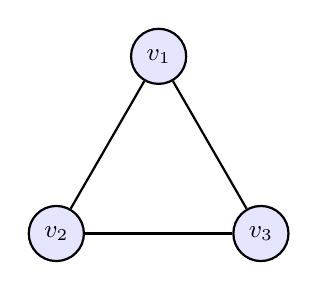
\begin{tikzpicture}[
    every node/.style={circle, draw, fill=blue!10, minimum size=0.7cm, font=\small},
    thick
]
    % Vértices distribuidos uniformemente en un círculo de radio 1.5
    \node (v1) at (90:1.5) {$v_1$};
    \node (v2) at (210:1.5) {$v_2$};
    \node (v3) at (330:1.5) {$v_3$};
    
    % Aristas que conectan todos los pares de vértices
    \draw (v1) -- (v2);
    \draw (v2) -- (v3);
    \draw (v3) -- (v1);
    \end{tikzpicture} 
    \end{figure}
    \noindent
    El conjunto $\{v_1\}$ es un CD pero no es un CV, pues la arista $(v_2,v_3)\in E$ no está dominada.\\

    \noindent
    Por otra parte, ¿todo CV es un CD? 
    \begin{prop}\label{prop}
        Sea $G=(V,E)$ un grafo sin vértices aislados, si $V'\subseteq V$ es un CV entonces $V'$ es un CD.
        \begin{proof}
            Sea $v\in V\setminus V'$, como $v$ es un vértice de $G$ y $G$ no tiene vértices aislados, entonces debe existir $e\in E$ de forma que $e$ conecte $v$ con otro vértice $u\in V$. Como $V'$ es un CV debemos tener que $u\in V'$.
        \end{proof}
    \end{prop}
    \noindent
    La hipótesis extra de que $G$ sea un grafo sin vértices aislados se debe a que en un grafo cualquiera $G$ debemos asegurarnos de que un CV $V'$ contiene todos los vértices aislados para poder asegurar que es un CD.
    \begin{ejemplo}
        En el siguiente grafo tenemos que $\{v_2\}$ es un CV pero no un CD, puesto que no domina al vértice $v_1$. Para transformar este CV en un CD debemos incluir el vértice $v_1$: $\{v_1,v_2\}$ sí es un CD.
        \begin{figure}[H]
            \centering
        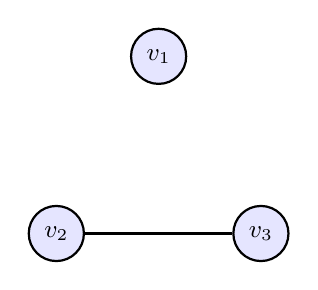
\begin{tikzpicture}[
        every node/.style={circle, draw, fill=blue!10, minimum size=0.7cm, font=\small},
        thick
    ]
        % Vértices distribuidos uniformemente en un círculo de radio 1.5
        \node (v1) at (90:1.5) {$v_1$};
        \node (v2) at (210:1.5) {$v_2$};
        \node (v3) at (330:1.5) {$v_3$};
        
        % Aristas que conectan todos los pares de vértices
        \draw (v2) -- (v3);
        \end{tikzpicture} 
        \end{figure}
    \end{ejemplo}

    \noindent
    La Proposición~\ref{prop} nos ayuda bastante a la hora de probar que \CD es un problema NP-completo, pues buscamos un algoritmo ALG(G, J) $\in$ L de modo que:
    \begin{center}
        SÍ = \CV $\quad\Longleftrightarrow\quad $ SÍ = CD(ALG(G, J))
    \end{center}
    Con ayuda de la Proposición tenemos que si $G$ no tiene vértices aislados entonces:
    \begin{center}
        SÍ = \CV $\quad\Longrightarrow\quad$ SÍ = CD(G, J)
    \end{center}
    Así, basta buscar una estrategia (modificaciones espacio-logarítmicas sobre $G$ y $J$) para ver que si NO = \CV entonces NO = CD($G'$, $J'$), sin perder la propiedad superior.\\

    \noindent
    Así, si NO = \CV entonces no existe un recubrimiento por vértices de $G$ de menos de $J$ vértices, es decir:
    \begin{equation*}
        \forall V'\subseteq V ~:~ |V'| \leq J ~~\exists (u,v)\in E~~\text{con}~~u,v\notin V'
    \end{equation*}
    Bajo estas hipótesis, ¿cómo aseguramos que $G'$ no tenga un CD? Si a cada arista $(u,v)\in E$ añadimos un nuevo vértice que solo se conecte con $u$ y $v$, y mantenemos $J' = J$:
    \begin{figure}[H]
        \centering
    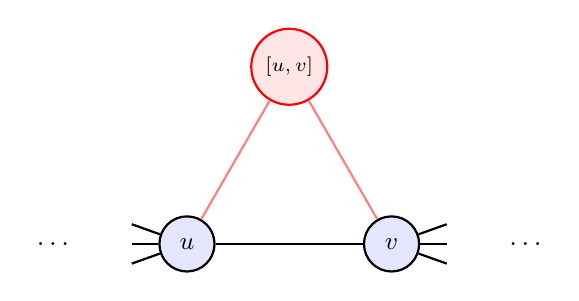
\begin{tikzpicture}[
    vertex/.style={circle, draw, fill=blue!10, minimum size=0.7cm, font=\small},
    thick
]
    % Vértices distribuidos uniformemente en un círculo de radio 1.5
    \node[vertex, font=\scriptsize, fill=red!10, draw=red] (v1) at (90:1.5) {$[u,v]$};
    \node[vertex] (v2) at (210:1.5) {$u$};
    \node[vertex] (v3) at (330:1.5) {$v$};
    
    % Aristas que conectan todos los pares de vértices
    \draw[red!50] (v1) -- (v2);
    \draw (v2) -- (v3);
    \draw[red!50] (v3) -- (v1);
    \draw (v2) -- (-2,-0.5);
    \draw (v2) -- (-2,-0.75);
    \draw (v2) -- (-2,-1);
    \draw (v3) -- (2,-0.75);
    \draw (v3) -- (2,-0.5);
    \draw (v3) -- (2,-1);
    \node at (-3,-0.75) {$\dots$};
    \node at (3,-0.75) {$\dots$};
    \end{tikzpicture} 
    \end{figure}

    \noindent
    Como siempre tendremos la existencia de una arista que no sea dominada al no existir un CV, al añadir este nuevo nodo parece que es más difícil dominar todos los nodos. Además, si SÍ = \CV, entonces en cada $(u,v)\in E$ tendremos que bien $u\in V'$ o bien $v\in V'$, por lo que al añadir los vértices $[u,v]$ y si $G$ no tiene vértices aislados tendremos que $V'$ será también un CD, por la Proposición~\ref{prop} y por dominar ahora a $[u,v]$ gracias a su vecindad con $u$ y $v$.

    \subsubsection{Demostración}
    \noindent
    Motivados todos los pasos que haremos, procedemos con la demostración rigurosa. Proponemos el algoritmo \ALG, que dados un grafo $G = (V,E)$ y $J\in \mathbb{N}$ con $J\leq |V|$ da como salida un nuevo grafo $G'$ y $K$ de modo que:
    \begin{itemize}
        \item $G'$ es el grafo obtenido tras aplicar al grafo $G$:
            \begin{itemize}
                \item Eliminar todos los vértices aislados de $G$.
                \item Para cada arista $(u,v)\in E$, añadir el nuevo nodo $[u,v]$ y las aristas $([u,v],u)$ y $([u,v],v)$.
            \end{itemize}
        \item $K = J$.
    \end{itemize}

    \begin{algorithm}
        \caption{}\label{alg2}
        \begin{algorithmic}
            \STATE \textbf{Entrada:} La codificación de un grafo $G=(V,E)$ y un número $J\leq |V|$ en binario.
            \STATE \textbf{Salida:} Se escribe en la cinta de salida un grafo $G'$ y un número $K$ en binario.\\

            \noindent
            \STATE \textbf{Para cada} $v\in V$ \textbf{hacer}
            \STATE \quad Guardar el índice de la casilla donde empieza $v$ en binario: $i_v$.
            \STATE \quad \texttt{aislado} = \textbf{true}\\

            \noindent
            \STATE \quad \textbf{Para cada} $(u,w)\in E$ \textbf{y mientras} \texttt{aislado} = \textbf{true} \textbf{hacer}
            \STATE \quad \quad Guardar el índice de la casilla donde empieza $(u, w)$ en binario: $i_{copia}$.
            \STATE \quad \quad \textbf{Si} $v = u$ \textbf{ó} $v = w$ \textbf{entonces} \texttt{aislado} = \textbf{false}
            \STATE \quad \textbf{Fin Para}\\

            \noindent
            \STATE \quad \textbf{Si} \texttt{aislado} = \textbf{false} \textbf{entonces}
            \STATE \quad \quad Escribir $v$ en la cinta de salida.
            \STATE \quad \textbf{Fin Si}
            \STATE \textbf{Fin Para}\\

            \noindent
            \STATE \textbf{Para cada} $(u,v)\in E$ \textbf{hacer}
            \STATE \quad Guardar en $i_{copia}$ el índice donde empieza $(u,v)$ en binario.
            \STATE \quad Escribir $[u, v]$ en la cinta de salida como un vértice de $G'$.
            \STATE \textbf{Fin Para}\\

            \noindent
            \STATE \textbf{Para cada} $(u,v)\in E$ \textbf{hacer}
            \STATE \quad Guardar en $i_{copia}$ el índice donde empieza $(u,v)$ en binario.
            \STATE \quad Escribir $(u, v)$ en la cinta de salida como una arista de $G'$.
            \STATE \quad Escribir $([u, v], u)$ en la cinta de salida como una arista de $G'$.
            \STATE \quad Escribir $([u, v], v)$ en la cinta de salida como una arista de $G'$.
            \STATE \textbf{Fin Para}\\

            \noindent
            \STATE Guardar en $i_{copia}$ el índice donde empieza $J$.
            \STATE Copiar $J$ en la cinta de salida como $K$.
        \end{algorithmic}
    \end{algorithm}

    \noindent
    El espacio empleado en \ALG es constante, salvo el empleado para almacenar los índices $i_v$ e $i_{copia}$. Estos son índices que referencian en binario posiciones a lo largo de la cinta de entrada, por lo que ocupan un espacio logarítmico. Así, tenemos que \ALG $\in L$.\\

    \noindent
    Ahora, hemos de comprobar que:
    \begin{center} 
        \CV = CD(ALG(G, J)) $\qquad \forall$ grafo $G=(V,E), \quad \forall J\leq |V|$
    \end{center}
    Para ello, sea $G=(V,E)$ un grafo y $J\in \mathbb{N}$ con $J\leq |V|$, distinguimos casos:\\

    \noindent
    \textbf{Si \CV = SÍ}\newline
    En este caso tenemos que $\exists \cc{V}\subseteq V$ con $|\cc{V}|\leq J$ de forma que:
    \begin{equation*}
        \forall (u,v)\in E~~u\in \cc{V}\lor v\in \cc{V}
    \end{equation*}
    Sea $\overline{V}$ el conjunto de todos los vértices aislados de $V$:
    \begin{equation*}
        \overline{V} = \{v\in V : \nexists e\in E, u\in V \text{\ con\ } e = (u,v) \lor e = (v,u)\}
    \end{equation*}
    Por la definición de cubrimiento por vértices vemos que $\cc{V}' = \cc{V}\setminus \overline{V}$ seguirá siendo un CV de $G$ con $|\cc{V}'|\leq |\cc{V}|\leq J$, y también lo será del grafo $(V\setminus \overline{V},E)$, que no tiene vértices aislados, por lo que $\cc{V}'$ es un CD de este grafo gracias a la Proposición~\ref{prop}.\\

    \noindent
    Sea ahora $(G',K) = \ALG$, vemos que $(V\setminus \overline{V}, E)$ es un subgrafo del grafo $G' = (V',E')$, por lo que para que $\cc{V}'$ sea un CD de $G'$ basta ver que los vértices de la forma $[u,v]$ están dominados por $\cc{V'}$.\\

    \noindent
    Para ello, si $[u,v]\in V'$ debe existir por su construcción $(u,v)\in E$, y como $\cc{V}'$ es CV de $G$ debemos tener:
    \begin{itemize}
        \item bien $u\in \cc{V}'$, con lo que $[u,v]$ queda dominado por $u$ al tener $([u,v],u)\in E'$.
        \item bien $v\in \cc{V}'$, con lo que $[u,v]$ queda dominado por $v$ al tener $([u,v],u)\in E'$.
    \end{itemize}
    Así, acabamos de probar que $\cc{V}'$ es un CD de $G'$ con $|\cc{V}'|\leq J = K$, con lo que podemos afirmar que:
    \begin{center}
        SÍ = CD($G'$, K) = CD(\ALG)
    \end{center}

    \noindent
    \textbf{Si \CV = NO}\newline
    Tenemos que $\nexists \cc{V}\subseteq V$ con $|\cc{V}|\leq J$ de forma que:
    \begin{equation*}
        \forall (u,v)\in E~~u\in \cc{V}\lor v\in \cc{V}
    \end{equation*}
    Es decir, $\forall \cc{V}\subseteq V$ con $|\cc{V}|\leq J$ se tiene que:
    \begin{equation*}
        \exists (u,v)\in E~~u,v\in V\setminus \cc{V}
    \end{equation*}
    Sea $(G',K) = \ALG$, tenemos $G'=(V',E')$. Por \underline{reducción al absurdo}, supongamos que:
    \begin{equation*}
        \exists \cc{V}'\subseteq V' \text{\ con\ } |\cc{V}'|\leq J \text{\ CD de\ } G'
    \end{equation*}
    Podemos considerar ahora:
    \begin{equation*}
        \overline{\cc{V}} = \cc{V}' \setminus \{[u,v] \in V' : (u,v)\in E\}\subseteq V
    \end{equation*}
    con $|\overline{\cc{V}}|\leq |\cc{V}'|\leq J$, por lo que por hipótesis (no existe CV de $G$) sabemos que $\exists (u,v)\in E$ con $u,v\in V\setminus \overline{\cc{V}}$. Además, por ser $E$ un conjunto finito, debe existir una cantidad finita de dichos arcos, $B\in \mathbb{N}$, que podemos agrupar en el conjunto:
    \begin{equation*}
        \Lambda = \left\{(u,v)\in E : u,v\in V\setminus \overline{V}\right\}
    \end{equation*}

    \noindent
    De $u,v\in V\setminus \overline{\cc{V}}$ deducimos que $u,v\notin \cc{V}'$. Ahora, como $\cc{V}'$ es un CD de $G'$ y los vértices adyacentes a $[u,v]\in V'$ solo son $u$ y $v$ deducimos que debemos tener $[u,v]\in \cc{V}'$. De esta forma, en realidad teníamos que $|\overline{\cc{V}}|\leq J-1$ (pues $\overline{\cc{V}}$ no puede contener a $[u,v]$). Este mismo razonamiento podemos repetirlo para cada elemento de $\Lambda$, obteniendo así que en realidad:
    \begin{equation*}
        |\overline{\cc{V}}| \leq J-B
    \end{equation*}
    Ahora, definimos:
    \begin{equation*}
        \widetilde{\cc{V}} = \overline{\cc{V}} \cup \{u \in V : \exists v\in V \text{\ con\ } (u,v)\in \Lambda\} \subseteq V
    \end{equation*}
    Observemos que $\widetilde{\cc{V}}$ es un CV de $G$, ya que si $(u,v)\in E$ tenemos dos opciones:
    \begin{itemize}
        \item Bien $u\in \overline{\cc{V}}$ ó $v\in \overline{\cc{V}}$, por lo que $(u,v)$ queda dominada por $\widetilde{\cc{V}}$.
        \item Bien $u,v\in V\setminus \overline{\cc{V}}$, pero entonces tenemos que $(u,v)\in \Lambda$, de donde $u\in \widetilde{\cc{V}}$ por definición.
    \end{itemize}
    Pero también de $|\overline{\cc{V}}|\leq J-B$ y de $|\Lambda| = B$ deducimos que $|\widetilde{\cc{V}}| \leq J$, hemos llegado a una \underline{contradicción}, pues $G$ no podía tener ningún CV de menos de $J$ vértices. Acabamos de probar que:
    \begin{equation*}
        \nexists \cc{V}'\subseteq V' \text{\ con\ } |\cc{V}'|\leq J \text{\ CD de\ } G'
    \end{equation*}
    Es decir, que:
    \begin{center}
        NO = CD($G'$, K) = CD(\ALG)
    \end{center}~\\
    Así, acabamos de probar que:
    \begin{equation*}
        \boxed{\CV \propto \CD} 
    \end{equation*}
    Por lo que \CD es NP-completo, ya que \CV es NP-Completo.
\end{document}


